\documentclass{article}
\usepackage{amsmath}
\usepackage{tikz}
\usepackage{circuitikz}
\usepackage{pgf}

\begin{document}

\section*{Versuch 5: Synchrone Schaltwerke und Automaten}

\subsection*{a. Synchroner Modulo-7-Zähler als Medwedew-Automat}

\subsubsection*{Zustandsgraph und Notation}
Zustände: \(0, 1, 2, 3, 4, 5, 6\)

\[
\begin{aligned}
&0 \rightarrow 1 \rightarrow 2 \rightarrow 3 \rightarrow 4 \rightarrow 5 \rightarrow 6 \rightarrow 0
\end{aligned}
\]

\subsubsection*{Zustandsfolgetabelle}

\begin{tabular}{|c|c|c|c|}
\hline
\text{Zustand (Z)} & D2 & D1 & D0 \\
\hline
000 & 0 & 0 & 1 \\
001 & 0 & 1 & 0 \\
010 & 0 & 1 & 1 \\
011 & 1 & 0 & 0 \\
100 & 1 & 0 & 1 \\
101 & 1 & 1 & 0 \\
110 & 0 & 0 & 0 \\
\hline
\end{tabular}

\subsubsection*{KV-Diagramme und Minimierung}

Für \(D2\):

\begin{tabular}{|c|c|c|c|c|}
\hline
 & 00 & 01 & 11 & 10 \\
\hline
0 & 0 & 0 & 1 & 1 \\
1 & x & x & x & x \\
\hline
\end{tabular}

\[
D2 = Z1 \cdot Z0
\]

Für \(D1\):

\begin{tabular}{|c|c|c|c|c|}
\hline
 & 00 & 01 & 11 & 10 \\
\hline
0 & 0 & 1 & 1 & 0 \\
1 & x & x & x & x \\
\hline
\end{tabular}

\[
D1 = \overline{Z1} \cdot Z0 + Z1 \cdot \overline{Z0}
\]

Für \(D0\):

\begin{tabular}{|c|c|c|c|c|}
\hline
 & 00 & 01 & 11 & 10 \\
\hline
0 & 1 & 0 & 1 & 0 \\
1 & x & x & x & x \\
\hline
\end{tabular}

\[
D0 = \overline{Z0}
\]

\subsubsection*{Logikplan}

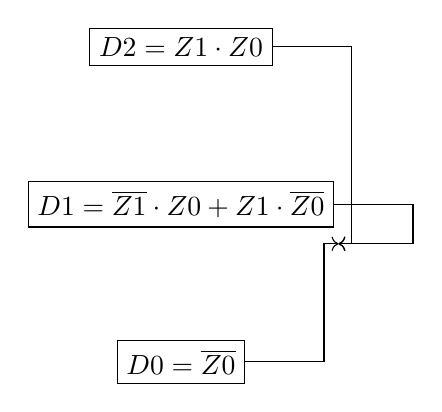
\begin{tikzpicture}
    \node[draw, rectangle] (D2) at (0,0) {$D2 = Z1 \cdot Z0$};
    \node[draw, rectangle] (D1) at (0,-2) {$D1 = \overline{Z1} \cdot Z0 + Z1 \cdot \overline{Z0}$};
    \node[draw, rectangle] (D0) at (0,-4) {$D0 = \overline{Z0}$};
    \draw[->] (D2.east) -- ++(1,0) |- (2,-2.5);
    \draw[->] (D1.east) -- ++(1,0) |- (2,-2.5);
    \draw[->] (D0.east) -- ++(1,0) |- (2,-2.5);
\end{tikzpicture}

\subsection*{b. Steuerbarer, synchroner Zähler mit einstellbarer Zählfolge}

\subsubsection*{Zustandsfolgetabelle}

Für \(S = 0\):

\begin{tabular}{|c|c|c|c|}
\hline
\text{Zustand (Z)} & \text{JK-FF Q2} & \text{JK-FF Q1} & \text{JK-FF Q0} \\
\hline
000 & 0 & 0 & 1 \\
001 & 0 & 1 & 0 \\
010 & 0 & 1 & 1 \\
011 & 1 & 0 & 0 \\
100 & 1 & 0 & 1 \\
\hline
\end{tabular}

Für \(S = 1\):

\begin{tabular}{|c|c|c|c|}
\hline
\text{Zustand (Z)} & \text{JK-FF Q2} & \text{JK-FF Q1} & \text{JK-FF Q0} \\
\hline
000 & 0 & 0 & 1 \\
001 & 0 & 1 & 1 \\
011 & 1 & 0 & 0 \\
100 & 1 & 0 & 1 \\
010 & 0 & 0 & 0 \\
\hline
\end{tabular}

\subsubsection*{KV-Diagramme und Minimierung}
Die KV-Diagramme für die Ansteuersignale der JK-Flipflops werden erstellt und minimiert.

\subsubsection*{Logikplan}

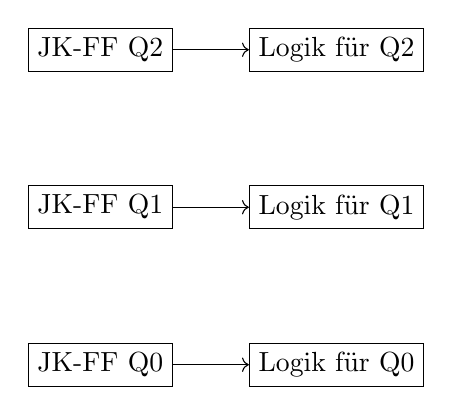
\begin{tikzpicture}
    \node[draw, rectangle] (JK2) at (0,0) {JK-FF Q2};
    \node[draw, rectangle] (JK1) at (0,-2) {JK-FF Q1};
    \node[draw, rectangle] (JK0) at (0,-4) {JK-FF Q0};
    \node[draw, rectangle] (Logic2) at (3,0) {Logik für Q2};
    \node[draw, rectangle] (Logic1) at (3,-2) {Logik für Q1};
    \node[draw, rectangle] (Logic0) at (3,-4) {Logik für Q0};
    \draw[->] (JK2.east) -- (Logic2.west);
    \draw[->] (JK1.east) -- (Logic1.west);
    \draw[->] (JK0.east) -- (Logic0.west);
\end{tikzpicture}

\subsection*{c. Steuerung einer Straßen-Baustellen-Absicherung als Moore-Automat}

\subsubsection*{Zustandsfolgetabelle}

\begin{tabular}{|c|c|c|c|c|}
\hline
\text{Zustand (Z)} & \text{JK-FF A3} & \text{JK-FF A2} & \text{JK-FF A1} & \text{JK-FF A0} \\
\hline
0 & 0 & 0 & 0 & 1 \\
1 & 0 & 0 & 1 & 0 \\
2 & 0 & 1 & 0 & 0 \\
3 & 1 & 0 & 0 & 0 \\
4 & 0 & 0 & 0 & 0 \\
\hline
\end{tabular}

\subsubsection*{KV-Diagramme und Minimierung}
Die KV-Diagramme für die Übergangs- und Ausgangsfunktionen werden erstellt und minimiert.

\subsubsection*{Logikplan}

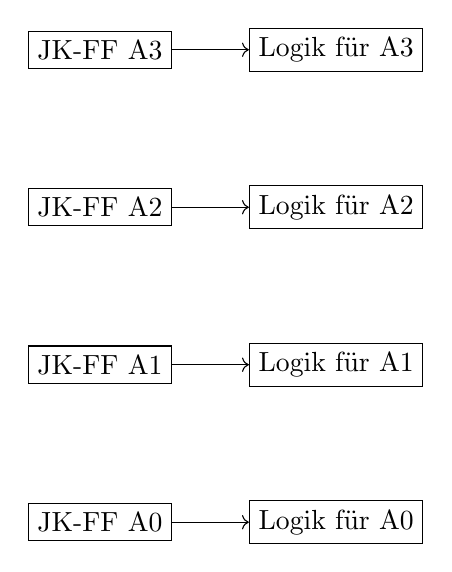
\begin{tikzpicture}
    \node[draw, rectangle] (JK3) at (0,0) {JK-FF A3};
    \node[draw, rectangle] (JK2) at (0,-2) {JK-FF A2};
    \node[draw, rectangle] (JK1) at (0,-4) {JK-FF A1};
    \node[draw, rectangle] (JK0) at (0,-6) {JK-FF A0};
    \node[draw, rectangle] (Logic3) at (3,0) {Logik für A3};
    \node[draw, rectangle] (Logic2) at (3,-2) {Logik für A2};
    \node[draw, rectangle] (Logic1) at (3,-4) {Logik für A1};
    \node[draw, rectangle] (Logic0) at (3,-6) {Logik für A0};
    \draw[->] (JK3.east) -- (Logic3.west);
    \draw[->] (JK2.east) -- (Logic2.west);
    \draw[->] (JK1.east) -- (Logic1.west);
    \draw[->] (JK0.east) -- (Logic0.west);
\end{tikzpicture}

\section*{Versuch 6: Programmzähler und Serienaddierwerk}

\subsection*{a. 3-Bit-Befehlszähler}

\subsubsection*{Zustandsfolgetabelle ohne Ladefunktion}

\begin{tabular}{|c|c|c|c|}
\hline
\text{Zustand (Z)} & D2 & D1 & D0 \\
\hline
000 & 0 & 0 & 1 \\
001 & 0 & 1 & 0 \\
010 & 0 & 1 & 1 \\
011 & 1 & 0 & 0 \\
100 & 1 & 0 & 1 \\
101 & 1 & 1 & 0 \\
110 & 1 & 1 & 1 \\
111 & 0 & 0 & 0 \\
\hline
\end{tabular}

\subsubsection*{KV-Diagramme und Minimierung}
Die KV-Diagramme für die Flipflop-Ansteuersignale werden erstellt und minimiert.

\subsubsection*{Logikplan}

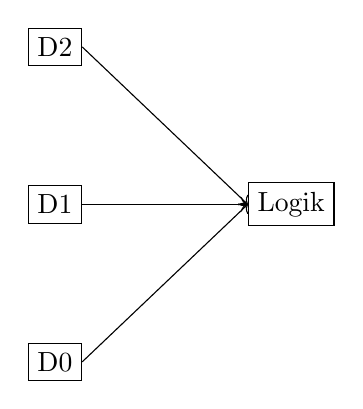
\begin{tikzpicture}
    \node[draw, rectangle] (D2) at (0,0) {D2};
    \node[draw, rectangle] (D1) at (0,-2) {D1};
    \node[draw, rectangle] (D0) at (0,-4) {D0};
    \node[draw, rectangle] (Logic) at (3,-2) {Logik};
    \draw[->] (D2.east) -- (Logic.west);
    \draw[->] (D1.east) -- (Logic.west);
    \draw[->] (D0.east) -- (Logic.west);
\end{tikzpicture}

\subsection*{b. Serienaddierwerk}

\subsubsection*{Logikplan}
Der Logikplan für das Serienaddierwerk wird erstellt.

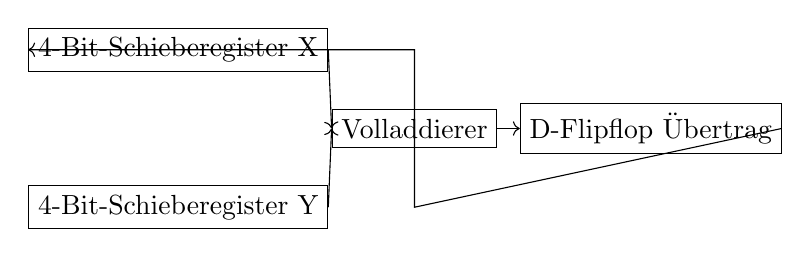
\begin{tikzpicture}
    \node[draw, rectangle] (X) at (0,0) {4-Bit-Schieberegister X};
    \node[draw, rectangle] (Y) at (0,-2) {4-Bit-Schieberegister Y};
    \node[draw, rectangle] (FA) at (3,-1) {Volladdierer};
    \node[draw, rectangle] (Carry) at (6,-1) {D-Flipflop Übertrag};
    \draw[->] (X.east) -- (FA.west);
    \draw[->] (Y.east) -- (FA.west);
    \draw[->] (FA.east) -- (Carry.west);
    \draw[->] (Carry.east) -- (3,-2) |- (X.west);
\end{tikzpicture}

\subsubsection*{Funktionsüberprüfung}
Die Funktion der Schaltung wird überprüft.

\end{document}
